\chapter{Einstellungen}\label{einstellungen}
Im Menü "`Einsatzplaner"' haben Sie unter dem Eintrag "`Einstellungen \dots"' die Möglichkeit Einstellungen für das Programm festzulegen (siehe Abbildung~\ref{fig:einstellungen}).
\begin{figure}[!h]
	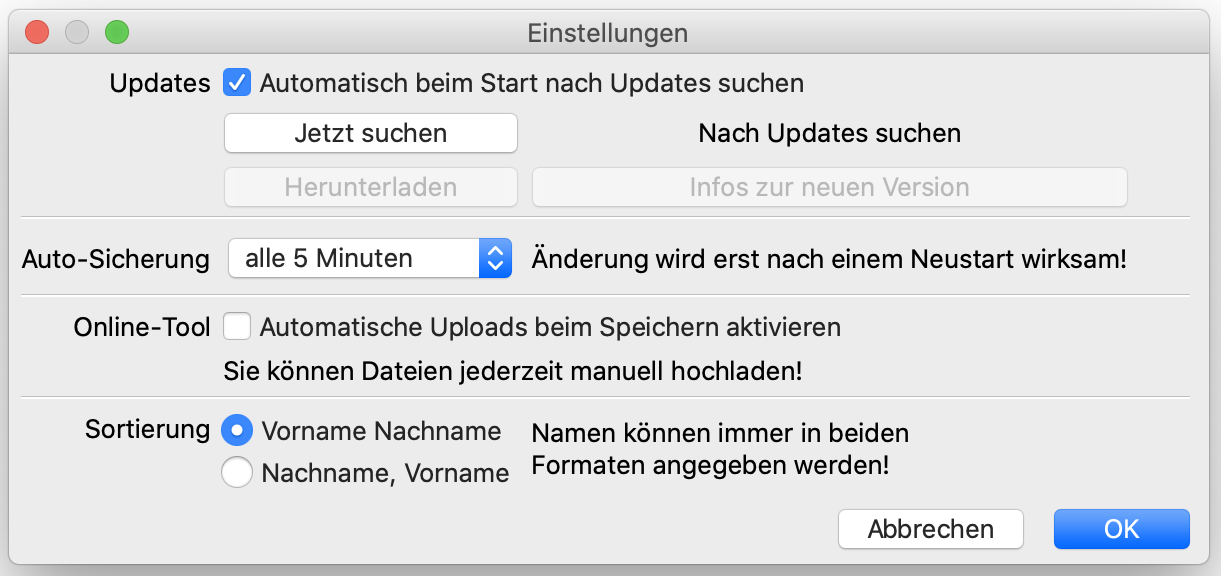
\includegraphics[width=\textwidth]{img/einstellungen}
	\caption{Das Fenster für die Programmeinstellungen.}
	\label{fig:einstellungen}
\end{figure}



\section{Updates}
Sie können eine automatische Suche nach neuen Versionen des Programms einstellen.
Ebenso können Sie sich die Informationen zur aktuellen Programmversion ansehen.

Die Funktion ist standardmäßig aktiviert.



\section{Auto-Sicherung}
Hier haben Sie die Möglichkeit einzustellen, ob das Program eine automatische Sicherung durchführen soll.
Bei dieser Funktion wird ihre originale Datei nicht überschrieben.
Stattdessen wird eine Datei mit dem gleichen Namen erstellt, der um \texttt{.autosave.ako} ergänzt ist.
Diese Datei wird automatische beim manuellen Speichern entfernt.
Sollte das Programm unerwartet abstürzen, können Sie diese Datei direkt öffnen.

Standardmäßig ist diese Funktion deaktiviert!



\section{Online-Tool}
Hier können Sie einstellen, ob beim manuellen Speichern eine Listenansicht auf den Server hochgeladen wird.
Dies setzt voraus, dass die entsprechende Option in den Einstellungen für die Einsatzplaner-Datei auch aktiviert ist
(siehe Kapitel~\ref{upload}).
Unabhängig von diesen Einstellungen können Sie die Ansicht jederzeit über die Exportfunktion (Kapitel~\ref{export:aktivitaeten}) hochladen.


\section{Anzeige Namen}
Es kann eingestellt werden, wie die Namen der Personen in der Mitgliederübersicht angezeigt und sortiert werden.
Die Änderung wird beim nächsten Aktualisieren der Mitgliederverwaltung wirksam und erfordert keinen Neustart.
